\documentclass{beamer}

\usepackage{graphicx, amssymb}
%\usepackage[active]{srcltx}
%\usepackage[all,xdvi]{xy}
%\usepackage{showlabels}
\usepackage[alphabetic,y2k,lite]{amsrefs}

%%%%%%%%%%%%%%%%%% Tikz %%%%%%%%%
\usepackage{tikz}
\usetikzlibrary{shapes.geometric}
\usetikzlibrary{calc}
\usetikzlibrary{scopes}
\usetikzlibrary{decorations.markings}
%\usepackage[labelformat=empty]{caption}

\tikzset{
every picture/.style={line width=0.8pt, >=stealth,
                       baseline=-3pt,label distance=-3pt},
%%%%%%%%%%  Node styles
dotnode/.style={fill=black,circle,minimum size=2.5pt, inner sep=1pt, outer
sep=0},
morphism/.style={circle,draw,thin, inner sep=1pt, minimum size=15pt,
                 scale=0.8},
small_morphism/.style={circle,draw,thin,inner sep=1pt,
                       minimum size=10pt, scale=0.8},
coupon/.style={draw,thin, inner sep=1pt, minimum size=18pt,scale=0.8},
%%%% different line styles:
regular/.style={densely dashed},
edge/.style={thick, dashed, draw=blue, text=black},
boundary/.style={thick,  draw=blue, text=black},
overline/.style={preaction={draw,line width=2mm,white,-}},
drinfeld center/.style={>=stealth,green!60!black, double
distance=1pt,text=black},
%%%%%%% Fill styles %%%%%%%%%%%%%%%
cell/.style={fill=black!10},
subgraph/.style={fill=black!30},
%%%%%%% Mid-path arrows
midarrow/.style={postaction={decorate},
                 decoration={
                    markings,% switch on markings
                    mark=at position #1 with {\arrow{>}},
                 }},
midarrow/.default=0.5
}
%%%%%%%%%%%%%%%%%%%%%%%%%%%%%%%%%%%%%%%%

\newcommand{\ph}{\varphi}
\renewcommand{\Im}{\mathrm{Im}}

\newcommand{\ee}{\mathbf{e}}
\DeclareMathOperator{\Obj}{Obj}
\DeclareMathOperator{\Hom}{Hom}
\DeclareMathOperator{\ev}{ev}
\DeclareMathOperator{\MCG}{MCG}
\DeclareMathOperator{\Homeo}{Homeo}
\DeclareMathOperator{\Vect}{Vect}
\DeclareMathOperator{\Mod}{Mod}
\DeclareMathOperator{\PGL}{PGL}

\newtheorem{proposition}[theorem]{Proposition}




% There are many different themes available for Beamer. A comprehensive
% list with examples is given here:
% http://deic.uab.es/~iblanes/beamer_gallery/index_by_theme.html
% You can uncomment the themes below if you would like to use a different
% one:
%\usetheme{AnnArbor}
%\usetheme{Antibes}
%\usetheme{Bergen}
%\usetheme{Berkeley}
%\usetheme{Berlin}
%\usetheme{Boadilla}
%\usetheme{boxes}
%\usetheme{CambridgeUS}
%\usetheme{Copenhagen}
%\usetheme{Darmstadt}
%\usetheme{default}
%\usetheme{Frankfurt}
%\usetheme{Goettingen}
%\usetheme{Hannover}
%\usetheme{Ilmenau}
%\usetheme{JuanLesPins}
%\usetheme{Luebeck}
\usetheme{Madrid}
%\usetheme{Malmoe}
%\usetheme{Marburg}
%\usetheme{Montpellier}
%\usetheme{PaloAlto}
%\usetheme{Pittsburgh}
%\usetheme{Rochester}
%\usetheme{Singapore}
%\usetheme{Szeged}
%\usetheme{Warsaw}

\title{Towards finiteness for mapping class group representations from group-theoretical categories}

% A subtitle is optional and this may be deleted
%\subtitle{Optional Subtitle}

\author{Paul Gustafson}%\inst{1}}
% - Give the names in the same order as the appear in the paper.
% - Use the \inst{?} command only if the authors have different
%   affiliation.

%\institute[Texas A\&M University] % (optional, but mostly needed)
%{
%  \inst{1}% 
%  Department of Mathematics \\
%  Texas A\&M University}
% - Use the \inst command only if there are several affiliations.
% - Keep it simple, no one is interested in your street address.

%\date{AMS Sectional on Fusion Categories and Topological Phases of Matter \\
% Salt Lake City, Utah \\
% April 2016}

\date{Preliminary Exam \\
May 2016}

% - Either use conference name or its abbreviation.
% - Not really informative to the audience, more for people (including
%   yourself) who are reading the slides online

%\subject{Theoretical Computer Science}
% This is only inserted into the PDF information catalog. Can be left
% out. 

% If you have a file called "university-logo-filename.xxx", where xxx
% is a graphic format that can be processed by latex or pdflatex,
% resp., then you can add a logo as follows:

% \pgfdeclareimage[height=0.5cm]{university-logo}{university-logo-filename}
% \logo{\pgfuseimage{university-logo}}

% Delete this, if you do not want the table of contents to pop up at
% the beginning of each subsection:
\AtBeginSubsection[]
{
  \begin{frame}<beamer>{Outline}
    \tableofcontents[currentsection,currentsubsection]
  \end{frame}
}

% Let's get started
\begin{document}

\begin{frame}
  \titlepage
\end{frame}

% Section and subsections will appear in the presentation overview
% and table of contents.


\begin{frame}{Definition of the mapping class group}
\begin{itemize}
\item
    Let $\Sigma = \Sigma_{g,b}^m$ be the oriented compact surface of genus $g$ with $b$ boundary components and $m$ marked points in its interior.

    \pause
\item
   The mapping class group of $\Sigma$, 
   $MCG(\Sigma),$
   is the group of isotopy classes of orientation-preserving homeomorphisms of $\Sigma$ that preserve the boundary \emph{pointwise} and preserve the marked points \emph{setwise}.
  
  \pause
  \item Examples
  \begin{itemize}
    \item $\MCG(\Sigma_{0,1}^m) = B_m$
    \item $\MCG(\Sigma_{1,0}^0) = SL(2,\mathbb Z)$
  \end{itemize}
\end{itemize}
\end{frame}

\begin{frame}{Introduction to the problem}

\begin{itemize}

\item In 2008, Etingof, Rowell, and Witherspoon \cite{erw} showed that the braid group representation associated to 
the modular category $\Mod(D^\omega(G))$ has finite image.

\pause \item They also asked if, more generally, all mapping class group representations associated to $\Mod(D^\omega(G))$ have 
finite image.

\pause \item In this talk, I'll work through the genus 2 case.
\end{itemize}
\end{frame}

\begin{frame}{Other Related Work}
%ng schaumburg - genus 1, any modular category
\begin{theorem}[Ng--Schauenberg \cite{Ng2010}]
Every modular representation associated to a modular category has finite image.
\end{theorem}

\pause 

\begin{theorem}[Fjelstad--Fuchs \cite{fjfu}]
Every mapping class group representation of a closed surface with at most one marked point associated to $\Mod(D(G))$ has finite image.
\end{theorem}

\begin{itemize}

\pause \item Fjelstad and Fuchs use Lyubashenko's method of constructing projective representations of mapping class groups from factorizable ribbon Hopf algebras (in this case $D(G)$).

\item We will use a different construction due to Kirillov.  In our case, this construction corresponds to the twisted Dijkgraaf-Witten theory.

\end{itemize}

\end{frame}

\begin{frame}{Outline}
  \tableofcontents
  % You  might wish to add the option [pausesections]
\end{frame}


\section{Input data}

\begin{frame}{Input data}

    \begin{figure}[h]
    \centering
    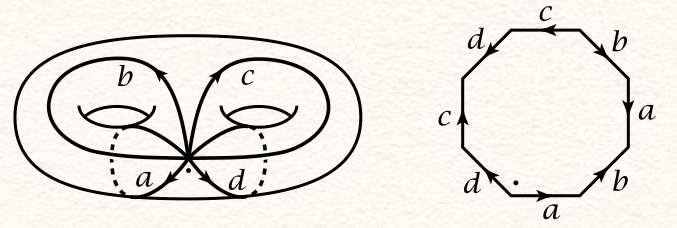
\includegraphics[width=0.8\textwidth, keepaspectratio]{hatcher-genus-2.jpg}
    \caption{A genus 2 surface $\Sigma$ as a quotient of its fundamental polygon. 
    Image source: Hatcher's \emph{Algebraic Topology}.}
    \end{figure}

  \begin{itemize}
  \item { Oriented closed surface $\Sigma$ of genus $2$
    }
  \pause \item {
    Finite group $G$
  }
  \pause \item {
    Normalized 3-cocycle $\omega: G \times G \times G \to U(1)$.
  }
  \end{itemize}
\end{frame}


\section{Generators for the mapping class group}

\begin{frame}{Generators for the mapping class group}
  \begin{itemize}
        \item A theorem  of Lickorish \cite{lickorish1964finite}  implies that $\MCG(\Sigma)$ is generated by the Dehn twists $T_a, T_b, T_c, T_d, T_{a^{-1}d}$.  
  \end{itemize}
  
  \begin{figure}[h]
    \centering
    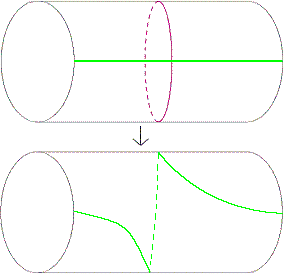
\includegraphics[height=0.4\textheight,keepaspectratio]{Dehn_twist.png}
    \caption{A Dehn twist with respect to the red curve. Image source: Wikipedia article on Dehn twists.}
    \end{figure}    
\end{frame}



\section{The representation space}

\begin{frame}{The representation space}
  \begin{itemize}
    \item 
        Using Kirillov's definitions \cite{kirillovStringNets}, the representation space is
        $$H := \frac{\text{$\Vect^\omega_G$-colored graphs in $\Sigma$}  }
    {\text{local relations}}$$
    \pause
    \item The vector space $H$ is canonically isomorphic to the Turaev-Viro state sum vector space 
    associated to $\Sigma$ \cite{kirillovStringNets}.  This isomorphism should commute with the mapping class group
    action.
    \pause \item  The Drinfel'd center $\mathcal Z (\Vect^\omega_G))$ is braided monoidally equivalent to
    $\Mod(D^\omega(G))$ (well-known according to \cite{0704.0195}).
    \pause \item Hence, the mapping class group representation on $H$ should be equivalent to the mapping class group representation 
    associated to $\Mod(D^\omega(G))$ by the Reshitikhin-Turaev construction \cite[preprint]{1012.0560}.
   \end{itemize}
\end{frame}

\begin{frame}{The spherical category $\Vect^\omega_G$}
\begin{itemize}
\item  The spherical fusion category $\Vect^\omega_G$ is the category of $G$-graded finite-dimensional vector spaces with the following
modified structural morphisms from \cite{math/0601012}, where $V_g$ is the simple object:   
\begin{itemize} 
\item The associator $a_{g,h,k}:(V_g \otimes V_h) \otimes V_k \to V_g \otimes (V_h \otimes V_k)$
            $$ a_{g,h,k} = \omega(g,h,k)$$
\item The evaluator $ev_g:V_g^* \otimes V_g \to 1$
            $$ ev_g = \omega(g^{-1},g,g^{-1})$$
\item The pivotal structure $j_g:V_g^{**} \to V_g$
            $$ j_g = \omega(g^{-1},g,g^{-1})$$
\end{itemize}
\end{itemize}
\end{frame}

\begin{frame}{Colored graphs in $\Sigma$}
\begin{itemize}
\item Let $\mathcal A$ be a spherical category (in our case, $\mathcal A = \Vect^\omega_G$).

\item Let $\Gamma \subset \Sigma$ be an undirected finite graph embedded in $\Sigma$.

\pause \item Define $E^{or}$ to be the set of orientation edges of $\Gamma$, i.e. pairs $\ee=(e,
\text{orientation of } e)$; for such an oriented edge $\ee$, we denote by $\bar{\ee}$ the edge with opposite orientation. 

\pause \item A {\em coloring} of $\Gamma$ is the
following data: 
\begin{itemize}
    \item Choice of an object $V(\ee)\in \Obj \mathcal A$ for every oriented edge  $\ee \in E^{or}$ so that $V(\bar{\ee})=V(\ee)^*$.
    \pause \item Choice of a vector $\ph(v)\in \Hom_{\mathcal A}(1, V_1 \otimes \cdots \otimes V_n)$  for  every interior vertex $v$, where 
      $\ee_1, \dots, \ee_n$ are edges incident to $v$, taken in counterclockwise 
      order and with outward orientation.
\end{itemize}
\end{itemize}
\end{frame}


\begin{frame}{Local relations}
\begin{itemize}
\item Isotopy of the graph embedding
\pause \item Linearity in the vertex colorings
\end{itemize}

\pause
\begin{figure}[ht]
%%%%%%%%%%%%%%%%%%%%%%%%%%%%%%%%%%%%%%%%%%%%%%%%%%%%%%%
%%%%%%%%%%

\begin{tikzpicture}
\node[morphism] (ph) at (0,0) {$\ph$};
\node[morphism] (psi) at (1,0) {$\psi$};
\node at (-0.7,0.1) {$\vdots$};
\node at (1.7,0.1) {$\vdots$};
\draw[->] (ph)-- +(220:1cm) node[pos=1.0,below,scale=0.8]
{$V_n$};
\draw[->] (ph)-- +(140:1cm) node[pos=1.0,above,scale=0.8]
{$V_1$};
\draw[->] (psi)-- +(40:1cm) node[pos=1.0,above,scale=0.8]
{$W_m$};
\draw[->] (psi)-- +(-40:1cm) node[pos=1.0,below,scale=0.8]
{$W_1$};
\draw[->] (ph) -- (psi) node[pos=0.5,above,scale=0.8] {$X$};
\end{tikzpicture}
%%%%%%%%
=
%%%%%%%%
\begin{tikzpicture}
\node[ellipse, thin, scale=0.8, inner sep=1pt, draw] (ph) at (0,0)
             {$\ph\circ_{X}\psi$};
\node at (-0.8,0.1) {$\vdots$};
\node at (0.8,0.1) {$\vdots$};
\draw[->] (ph)-- +(220:1cm) node[pos=1.0,below,scale=0.8] {$V_n$};
\draw[->] (ph)-- +(140:1cm) node[pos=1.0,above,scale=0.8] {$V_1$};
\draw[->] (ph)-- +(40:1cm) node[pos=1.0,above,scale=0.8]  {$W_m$};
\draw[->] (ph)-- +(-40:1cm) node[pos=1.0,below,scale=0.8] {$W_1$};
\end{tikzpicture}
%%%%%%%%%
\\
%%%%%%%%%
\begin{tikzpicture}
\node[dotnode] (ph) at (0,0) {};
\node[dotnode] (psi) at (1.5,0) {};
\node at (-0.7,0.1) {$\vdots$};
\node at (2.2,0.1) {$\vdots$};
\draw[->] (ph)-- +(220:1cm) node[pos=1.0,below,scale=0.8] {$A_n$};
\draw[->] (ph)-- +(140:1cm) node[pos=1.0,above,scale=0.8] {$A_1$};
\draw[->] (psi)-- +(40:1cm) node[pos=1.0,above,scale=0.8] {$B_m$};
\draw[->] (psi)-- +(-40:1cm) node[pos=1.0,below,scale=0.8] {$B_1$};
\draw[out=45,in=135, midarrow] (ph) to (psi)
                node[above,xshift=-0.6cm, yshift=0.25cm, scale=0.8] {$V_k$};
\draw[ out=15,in=165, midarrow] (ph) to (psi);
\draw[ out=-15,in=195, midarrow] (ph) to (psi);
\draw[ out=-45,in=225, midarrow] (ph) to (psi) node[below, xshift=-0.6cm, yshift=-0.3cm, scale=0.8] {$V_1$};
\end{tikzpicture}
%%%%%%%%%%%
=
%%%%%%%%%%%
\begin{tikzpicture}
\node[dotnode] (ph) at (0,0) {};
\node[dotnode] (psi) at (1.5,0) {};
\node at (-0.7,0.1) {$\vdots$};
\node at (2.2,0.1) {$\vdots$};
\draw[->] (ph)-- +(220:1cm) node[pos=1.0,below,scale=0.8] {$A_n$};
\draw[->] (ph)-- +(140:1cm) node[pos=1.0,above,scale=0.8] {$A_1$};
\draw[->] (psi)-- +(40:1cm) node[pos=1.0,above,scale=0.8] {$B_m$};
\draw[->] (psi)-- +(-40:1cm) node[pos=1.0,below,scale=0.8] {$B_1$};
\draw[ ->] (ph) to (psi)
            node[above,xshift=-0.8cm,scale=0.8] {$V_1\otimes \dots\otimes V_k$};
\end{tikzpicture}
%%%%%%%
\qquad $k\ge 0$
\\
%%%%%%%
\begin{tikzpicture}
\node[ellipse, scale=0.8, inner sep=1pt, draw,thin] (ph) at (0,0)
{$\mathrm{coev}$};
\draw[->] (ph)-- +(180:1cm) node[pos=1.0,above,scale=0.8] {$V$};
\draw[->] (ph)-- +(0:1cm) node[pos=1.0,above,scale=0.8] {$V^*$};
\end{tikzpicture}
%%%%%%%%
=
%%%%%%%%
\begin{tikzpicture}
\draw[->] (2,0)-- (0,0) node[pos=0.5,above,scale=0.8] {$V$};
\end{tikzpicture}
%%%%%%%%%%%%%%%%%%%%%%%%%%
\caption{The remaining local relations.
         Image source: \cite{kirillovStringNets}.
        }\label{f:local_rels1}
\end{figure}

\end{frame}

\begin{frame}{Consequences of the local relations}

\begin{figure}[ht]
%%%%%%%%%%%%
\begin{tikzpicture}
\node[morphism] (ph) at (0,0) {$\ph$};
\node[morphism] (psi) at (1.5,0) {$\psi$};
\node at (-0.7,0.1) {$\vdots$};
\node at (2.2,0.1) {$\vdots$};
\draw[->] (ph)-- +(220:1cm) node[pos=1.0,below,scale=0.8] {$V_n$};
\draw[->] (ph)-- +(140:1cm) node[pos=1.0,above,scale=0.8] {$V_1$};
\draw[->] (psi)-- +(40:1cm) node[pos=1.0,above,scale=0.8] {$W_m$};
\draw[->] (psi)-- +(-40:1cm) node[pos=1.0,below,scale=0.8] {$W_1$};
\draw[->] (ph) -- (psi) node[pos=0.5,above,scale=0.8] {$X_1\oplus X_2$};
\end{tikzpicture}
%%%%%%%%%%%%
=
%%%%%%%%%%%%
\begin{tikzpicture}
\node[morphism] (ph) at (0,0) {$\ph_1$};
\node[morphism] (psi) at (1.5,0) {$\psi_1$};
\node at (-0.7,0.1) {$\vdots$};
\node at (2.2,0.1) {$\vdots$};
\draw[->] (ph)-- +(220:1cm) node[pos=1.0,below,scale=0.8]{$V_n$};
\draw[->] (ph)-- +(140:1cm) node[pos=1.0,above,scale=0.8]{$V_1$};
\draw[->] (psi)-- +(40:1cm) node[pos=1.0,above,scale=0.8]{$W_m$};
\draw[->] (psi)-- +(-40:1cm) node[pos=1.0,below,scale=0.8]{$W_1$};
\draw[->] (ph) -- (psi) node[pos=0.5,above,scale=0.8] {$X_1$};
\end{tikzpicture}
%%%%%%%%%%%%
+
%%%%%%%%%%%%
\begin{tikzpicture}
\node[morphism] (ph) at (0,0) {$\ph_2$};
\node[morphism] (psi) at (1.5,0) {$\psi_2$};
\node at (-0.7,0.1) {$\vdots$};
\node at (2.2,0.1) {$\vdots$};
\draw[->] (ph)-- +(220:1cm) node[pos=1.0,below,scale=0.8]{$V_n$};
\draw[->] (ph)-- +(140:1cm) node[pos=1.0,above,scale=0.8]{$V_1$};
\draw[->] (psi)-- +(40:1cm) node[pos=1.0,above,scale=0.8]{$W_m$};
\draw[->] (psi)-- +(-40:1cm) node[pos=1.0,below,scale=0.8]{$W_1$};
\draw[->] (ph) -- (psi) node[pos=0.5,above,scale=0.8] {$X_2$};
\end{tikzpicture}
%%%%%%%%%%%%


\caption{Additivity in edge colorings. Here $\ph_1,\ph_2$ are compositions
of $\ph$ with projector $X_1\oplus X_2\to X_1$ (respectively, 
$X_1\oplus X_2\to X_2$), and similarly for $\psi_1,\psi_2$.
         Image source: \cite{kirillovStringNets}.
}
\end{figure}

\begin{itemize}
\item Additivity in edge colorings
\pause \item A colored graph may be evaluated on any disk $D\subset S$, giving
  an equivalent colored graph $\Gamma'$ such that $\Gamma'$ is identical
  to $\Gamma$ outside of $D$, has the same colored edges crossing $\partial D$,
  and contains at most one colored vertex within $D$.
\end{itemize}
\end{frame}


\section{A spanning set for the representation space}

\begin{frame}{A spanning set for the representation space}
\begin{figure}[h]
\centering
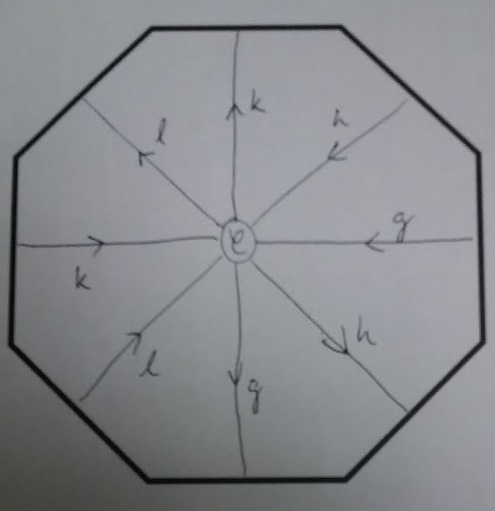
\includegraphics[height=0.5\textheight]{basis.jpg}
\caption{The spanning set $S$ consists of all such colored graphs, where the edge labels vary over all $4$-tuples $g,h,k,l \in G$ satisfying $[g,h][k,l] = 1$ and $\ph := \ph_{g,h,k,l}$ is the canonical basis element of the one-dimensional space $\Hom(1, (( \cdots ((V_g \otimes V_h) \otimes V_g^{-1}) \otimes \cdots \otimes V_l^{-1})$.}
\end{figure}
\end{frame}


\section{Action of the generators on the spanning set}
% You can reveal the parts of a slide one at a time
% with the \pause command:

\begin{frame}{Action of the Dehn twist $T_a$ on the spanning set \, I}
\begin{figure}[h]
\centering
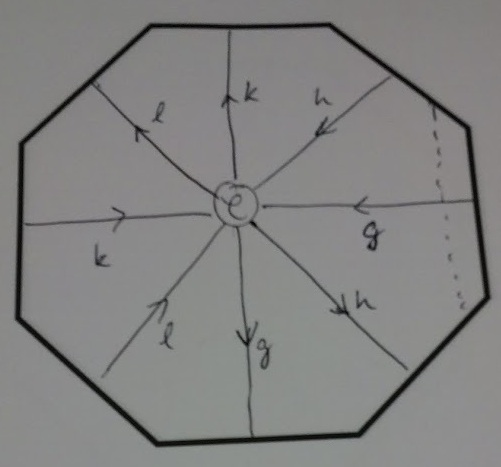
\includegraphics[height=0.7\textheight]{1.jpeg}
\caption{The dashed line is a simple closed curve isotopic to $a$.}
\end{figure}
\end{frame}


\begin{frame}{Action of the Dehn twist $T_a$ on the spanning set \, II}
\begin{figure}[h]
\centering
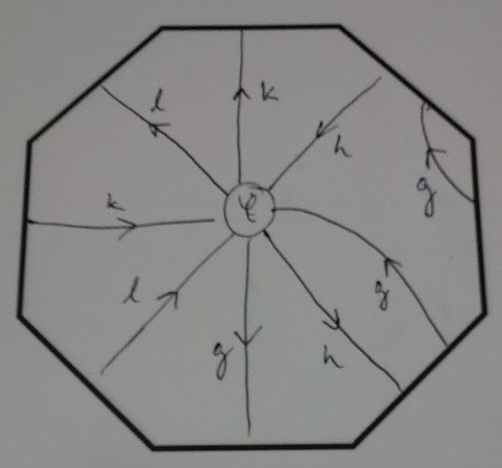
\includegraphics[height=0.7\textheight]{2.jpeg}
\caption{The result of the twist $T_a$.}
\end{figure}
\end{frame}


\begin{frame}{Action of the Dehn twist $T_a$ on the spanning set \, III}
\begin{figure}[h]
\centering
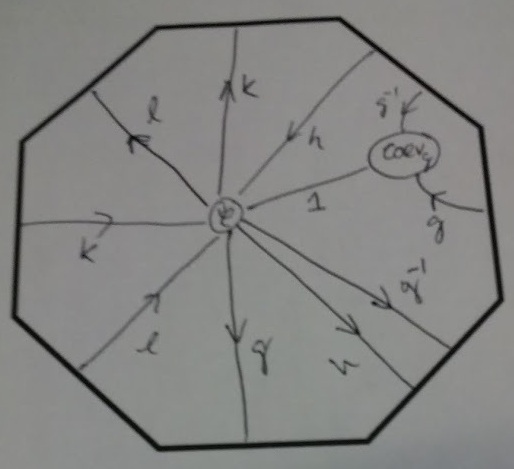
\includegraphics[height=0.7\textheight]{3.jpeg}
\caption{Using the local relations.}
\end{figure}
\end{frame}


\begin{frame}{Action of the Dehn twist $T_a$ on the spanning set \, IV}
\begin{figure}[h]
\centering
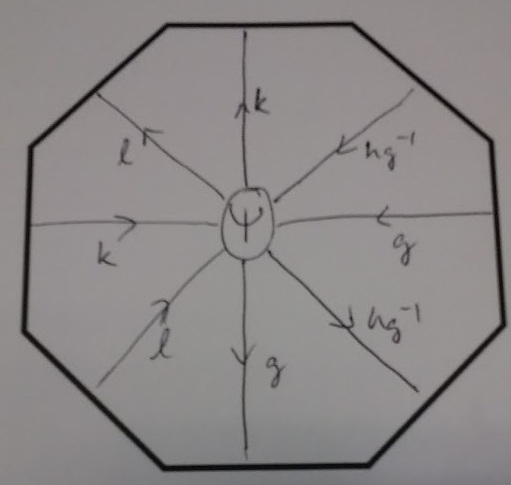
\includegraphics[height=0.7\textheight]{4.jpeg}
\caption{The result. The map $\psi$ differs from $\phi_{g,hg^{-1},k,l}$ by a product of factors in $\Im(\omega)$.}
\end{figure}
\end{frame}


\begin{frame}{Action of the Dehn twist $T_{a^{-1}d}$ on the spanning set \, I}
\begin{figure}[h]
\centering
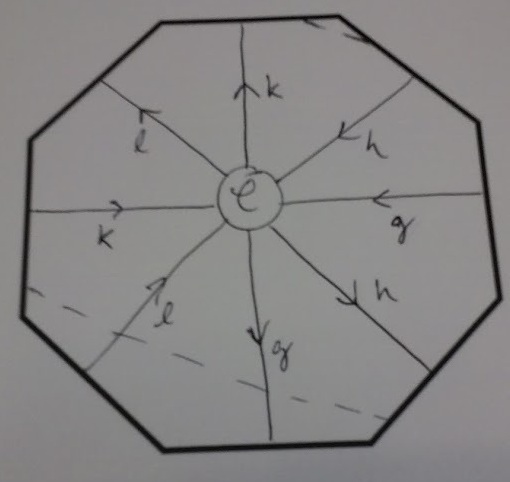
\includegraphics[height=0.7\textheight]{5.jpeg}
\caption{The dashed line is a simple closed curve isotopic to $a^{-1}d$.}
\end{figure}
\end{frame}


\begin{frame}{Action of the Dehn twist $T_{a^{-1}d}$ on the spanning set \, II}
\begin{figure}[h]
\centering
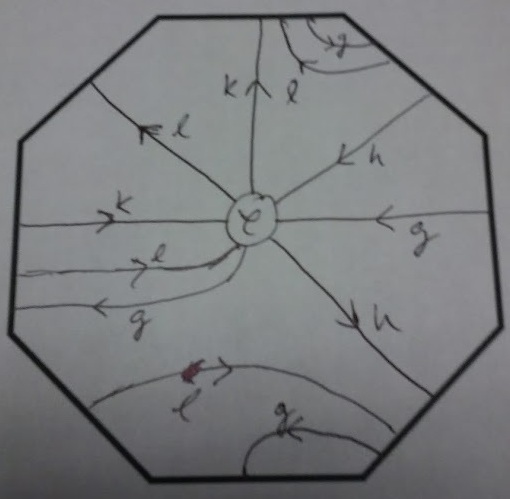
\includegraphics[height=0.7\textheight]{7.jpeg}
\caption{The result of the twist $T_{a^{-1}d}$.}
\end{figure}
\end{frame}


\begin{frame}{Action of the Dehn twist $T_{a^{-1}d}$ on the spanning set \, III}
\begin{figure}[h]
\centering
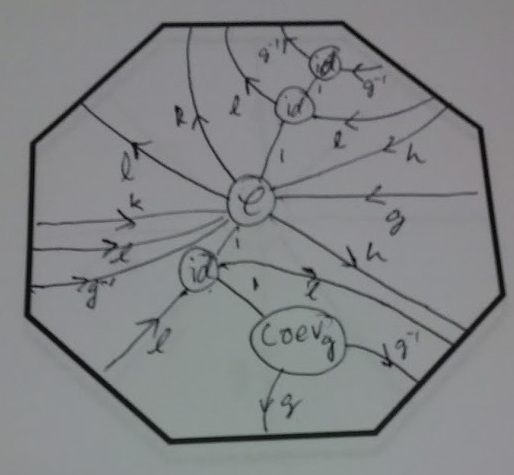
\includegraphics[height=0.7\textheight]{8.jpeg}
\caption{Using the local relations.}
\end{figure}
\end{frame}


\begin{frame}{Action of the Dehn twist $T_{a^{-1}d}$ on the spanning set \, IV}
\begin{figure}[h]
\centering
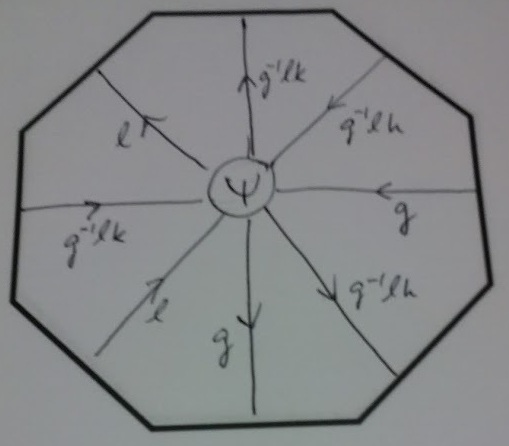
\includegraphics[height=0.7\textheight]{9.jpeg}
\caption{The result. Again, $\psi$ differs from $\phi_{g,g^{-1}lh,g^{-1}lk,l}$ by a product of factors in $\Im(\omega)$.}
\end{figure}
\end{frame}


\section{Sketch of a proof of finiteness}
\begin{frame}{Sketch of a proof of finiteness}
\begin{proposition}
Let $\rho: \MCG(\Sigma) \to \PGL(H)$ be the representation defined above.  Then $|\Im(\rho)| < \infty$. 
\end{proposition}

\emph{Sketch of proof.}  

\begin{itemize}
\item For any $k$, let $R$ denote the set of $|G|$-th roots of unity. Then $\omega$ is cohomologous to a cocycle taking values in $R$ (follows  from \cite[Theorem 6.58]{weibel1995introduction}).  Hence, WLOG $\omega$ takes values in $R$.

\pause \item  Let $L \subset \MCG(\Sigma)$ be the Lickorish generating set. From the previous slides,
$\rho(L) S \subset R S$. Hence $\rho(\MCG(\Sigma)) S \subset R S$. 

\pause \item Let $B \subset S$ be a basis for $H$. Then $\rho(\MCG(\Sigma)) B \subset \rho(\MCG(\Sigma)) S \subset R  S$.
 
 \pause \item   Thus, $|\Im(\rho)| < \infty$.
\end{itemize}
  
\end{frame}

\section{Future Directions}
\begin{frame}{Future Directions}
    \begin{itemize}
    \item Explicitly calculate the representation for low order abelian groups (in particular $\mathbb Z_3^3$). 
    \pause
    \item Add marked points using the Birman exact sequence.
    \pause 
    \item Look at the simplest undetermined cases of weakly integral modular categories.
    \end{itemize}
\end{frame}


\section*{Acknowledgements}
\begin{frame}{Acknowledgements}

\begin{itemize}
    \item Thanks to my advisor Eric Rowell, my father Robert Gustafson, and Zhenghan Wang for enlightening discussions.
    
    \pause \item Thanks for listening!
    \end{itemize}
\end{frame}

% All of the following is optional and typically not needed. 
%\appendix
%\section<presentation>*{\appendixname}
%\subsection<presentation>*{References}

\begin{frame}[allowframebreaks]
  \frametitle<presentation>{References}
  \bibliographystyle{unsrt}  
  \bibliography{stringnets}
\end{frame}

\end{document}


